\documentclass[mathserif, table]{beamer}

\usetheme{Boadilla}

\usepackage{subfig}
\usepackage{multirow}
\usepackage{xcolor,colortbl}
\usepackage{listings}
\usepackage{amsmath}

\lstset{language=C,tabsize=4, keepspaces=true,
    xleftmargin=2em,xrightmargin=2em, aboveskip=1em,
    backgroundcolor=\color{lightgray},    % 定义背景颜色
    frame=none,                      % 表示不要边框
    keywordstyle=\color{blue}\bfseries,
    breakindent=22pt,
    numbers=left,stepnumber=1,numberstyle=\tiny,
    basicstyle=\footnotesize,
    showspaces=false,
    flexiblecolumns=true,
    breaklines=true, breakautoindent=true,breakindent=4em,
    escapeinside={/*@}{@*/}
}

% Chinese
\usepackage{ctex}
\setCJKmainfont[BoldFont={SimHei},ItalicFont={KaiTi}]{KaiTi}

% Title
\title{第7章 离散模型的优化}
\author{韩建伟}
\institute{
  信息学院\\
  \texttt{mm@hanjianwei.com}
}
\date{2016/11/15}

\begin{document}

% Title page
\begin{frame}[plain]
  \titlepage{}
\end{frame}

\begin{frame}{数据拟合的准则}

  \begin{itemize}
  \item 切比雪夫近似准则
    \begin{itemize}
    \item 极小化$Maximum |y_i - f(x_i)|,  i = 1, 2, .., m$
    \item 线性规划问题
    \end{itemize}
  \item 极小化绝对偏差之和 
    \begin{itemize}
    \item 极小化$\sum_{i=1}^m |y_i - f(x_i)|$
    \item 前面没有给出具体的数学解法,7.6将会给出
    \end{itemize}
  \item 最小二乘准则 
    \begin{itemize}
    \item 极小化$\sum_{i=1}^m |y_i - f(x_i)|^2$
    \item 可以用微积分方法进行求解(第3,4章)
    \end{itemize}
  \end{itemize}
  
\end{frame}

\begin{frame}{用切比雪夫准则拟合直线}
  \begin{block}{问题}
    给定$m$个数据点$(x_i, y_i), i=1, 2, ..., m$,拟合一条直线$y=ax+b$(即确定参数$a, b$),使得所有数据点$(x_i, y_i)$和拟合直线上对应的点$(x_i, ax_i+b)$之间的距离的最大值$r_{max}$最小。也就是说,对整个这组数据点而言,最大绝对偏差$r=max\{|y_i-y(x_i)|\}$最小。
  \end{block}

  这种准则实际上定义了如下优化问题:
  \[ 
  \begin{array}{lcl}
    & & \mbox{Min}\ r \\
    \mbox{s.t.} & &  \\
    &
    \left.
      \begin{array}{c}
        r-r_i \ge 0\\
        r+r_i \ge 0
      \end{array}
    \right\}& i = 1, 2, ... , m
  \end{array}
  \]
\end{frame}

\begin{frame}{优化建模概述}

  \begin{block}{}
    \[ 
    \begin{array}{lcl}
      & \mbox{Opt}\ f_j(X) & j \in J\\
      \mbox{s.t.} & &  \\
      &
      g_i(X) \left\{
        \begin{array}{c}
          \ge\\
          = \\
          \le
        \end{array}
      \right\} b_i& i \in I
    \end{array}
    \]
  \end{block}
  \begin{itemize}
  \item $Opt$的意思是优化(最大或最小化),下标$j$指出优化目标可以是一个或多个函数,并用有限集合$J$的整数下标来区分
  \item 目标是找到向量$X_0$,使得函数$f_j(X)$取到最优值
  \item 向量$X$的各个分量称为该模型的\textbf{决策变量},$f_j(X)$称为\textbf{目标函数}
  \item ``s.t.''表示决策变量必须满足某些边界条件(即\textbf{约束}$g_i(X)$)
  \end{itemize}
  
\end{frame}

\begin{frame}{确定生产计划方案}
  \begin{block}{}
    木匠制作桌子和书架出售,成本分别为5美元和7美元。每周收益为:
    \[
    \begin{array}{cc}
      50x_1 - 0.2x_2^2, & x_1\text{为每周生产的桌子数量}\\
      65x_2 - 0.3x_2^2, & x_2\text{为每周生产的书架数量}
    \end{array}
    \]
    每周需制作多少桌子和书架才能使获得的利润最大?
  \end{block}
  
  利润函数:
  \[
  f(x_1, x_2) = 50x_1 - 0.2x_2^2 + 65x_2 - 0.3x_2^2 - 5x_1 - 7x_2
  \]

  \begin{itemize}
  \item 没有限定$x_1$, $x_2$的取值(可以是取值范围内的任意实数)
  \item 没有约束条件
  \item 是一个非线性表达式
  \end{itemize}
  
\end{frame}

\begin{frame}{木匠问题的变形}
  \begin{block}{}
木匠制作桌子和书架出售,单位净利润分别为25美元和30美元。他每周最多有690张木板可以用,每周最多工作120小时。生成一张桌子需要20张木板和5小时的劳动时间,生产一个书架需要30张木板和4小时的劳动时间。此外,他已经签订了每周供应4张桌子和2个书架的交货合同。每周需制作多少桌子和椅子才能使获得的利润最大?
  \end{block}

    \[ 
    \begin{array}{lcl}
      & \mbox{Max}\ 25x_1 + 30x_2 & \\
      \mbox{s.t.} & &  \\
      &
        \begin{array}{c}
          20x_1 + 30x_2 \le 690 (\text{木板})\\
          5x_1 + 4x_2 \le 120 (\text{劳动时间})\\
          x_1 \ge 4 (\text{合同})\\
          x_2 \ge 2 (\text{合同})
        \end{array}
        &
    \end{array}
    \]
  
\end{frame}

\begin{frame}{优化问题分类}
  \begin{description}
  \item[无约束] 没有约束条件
  \item[有约束] 有一个或多个边界条件
  \item[线性规划] 满足以下性质的称为线性规划:
    \begin{enumerate}
    \item 有唯一的目标函数
    \item 当一个决策变量出现在目标函数或者约束函数中时,它只以一次幂的形式出现(可以乘以一个常数)
    \item 目标函数和任何约束函数中不包含决策变量的乘积项
    \item 目标函数和任何约束函数中决策变量的系数是常数
    \item 决策变量的取值可以是整数,也可以是分数
    \end{enumerate}
  \end{description}
  
\end{frame}

\begin{frame}{优化问题的分类}
  \begin{itemize}
  \item 目标函数多于1个的称为\textbf{多目标或目标规划}
  \item 不满足2或者3的,称为\textbf{非线性规划}
  \item 如果不满足条件4,系数和时间相关的称为\textbf{动态规划}
  \item 如果不满足条件4,系数是随机的称为\textbf{随机规划}
  \item 如果决策变量限定为只能取整数,称为\textbf{整数规划},如果只限定部分决策变量为整数,称为\textbf{混合整数规划}
  \end{itemize}
\end{frame}

\begin{frame}{无约束优化问题}
  \begin{block}{绝对偏差之和问题}
    对模型$y=f(x)$,如果$y(x_i)$表示$x=x_i$点的函数值, $(x_i, y_i)表示对应的数据点, i=1, 2, ..., m$, 那么准则可以表示如下:找到模型$y=f(x)$,使得
    \[
    \mbox{Min} \sum_{i=1}^m |y_i - y(x_i)|
    \]
  \end{block}

  \begin{itemize}
  \item 无约束优化问题
  \item 由于被极小化函数的导数不连续,不能用微积分来解决(7.6节给出了基于模式搜索的数值解法
  \end{itemize}
  
\end{frame}

\begin{frame}{整数规划}
  \begin{block}{航天飞机载货问题}
    某航天飞机用于运载多种物品,遗憾的是,允许运载物品的重量和体积是有限制的。假设共有$m$件不同的物品,每件物品的价值为$c_j$,重量为$w_j$,体积为$v_j$。假定目标是在不超出重量限制$W$和体积限制$V$的条件下,最大化装载物品的价值。
  \end{block}
  令:
  \[
  y_i = \left\{
    \begin{array}{ll}
      1, & \text{如果物品$i$被装载}\\
      0, & \text{如果物品$i$不被装载}
    \end{array}
  \right.
  \]

  \begin{itemize}
  \item \textbf{0-1规划}
  \end{itemize}
\end{frame}

\begin{frame}{航天飞机载货问题}
  \[
  \mbox{Max}\ \sum_{j=1}^m c_jy_j
  \]
  s.t.
  \[
  \sum_{j=1}^m v_jy_j \le V
  \]
  \[
  \sum_{j=1}^m w_jy_j \le W
  \]

  \begin{itemize}
  \item 利用二进制变量可以表示是否的决策
  \item 也可用于某个变量的开关,如$x=ay, y=0\text{或}1$,则$x=0$或$x=a$
  \item 限定变量范围,如$ay < x < yb, y=0\text{或}1$, 则$a<x<b$或$x=0$
  \end{itemize}
  
\end{frame}

\begin{frame}{分段线性逼近}

  \begin{figure}
    \centering
    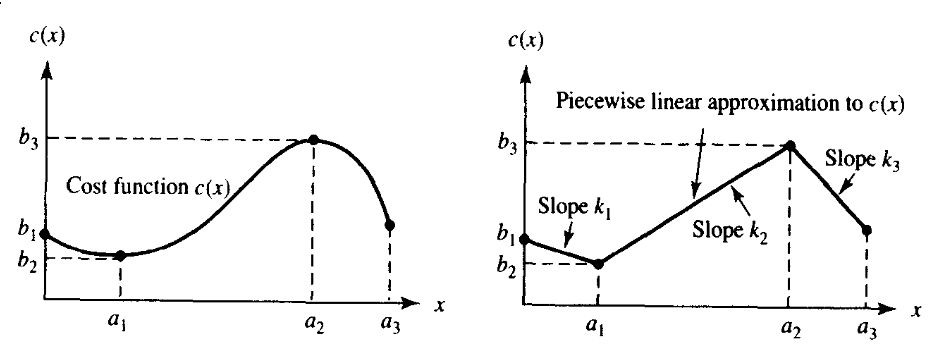
\includegraphics[width=.8\textwidth{}]{linear.png}
  \end{figure}

  \[
  c(x) =
  \left\{
    \begin{array}{ll}
      b_1 + k_1(x-0) & 0 \le x \le a_1 \\
      b_2 + k_2(x-a_1) & a_1 \le x \le a_2 \\
      b_3 + k_3(x-a_2) & a_2 \le x \le a_3 
    \end{array}
  \right.
  \]
\end{frame}

\begin{frame}{分段线性逼近}
  针对三个区间定义三个新的变量$x_1 = (x-0)$, $x_2 = (x-a_1)$, $x_3 = (x-a_2)$, 用二进制的变量$y_1$, $y_2$, $y_3$将$x_i$限定在对应的区间:
  \[
  \left.
    \begin{array}{l}
      0 \le x_1 \le y_1a_1 \\
      0 \le x_2 \le y_2(a_2 - a_1) \\
      0 \le x_3 \le y_3(a_3 - a_2)
    \end{array}
  \right.
  \]
  其中$y_1$, $y_2$, $y_3$等于0或1,因为任何情况下只能有一个$x$是有效的,所以有下面的约束:
  \[
  y_1 + y_2 + y_3 = 1
  \]
  注意到任何情况下只能有一个$x_i$是有效的,目标函数可以写成:
  \[
  c(x) = y_1(b_1 + k_1x_1) + y_2(b_2 + k_2x_2) + y_3(b_3 + k_3x_3)
  \]
\end{frame}

\begin{frame}{分段线性逼近}
  由于$y_i = 0$时,$x_i = 0$,因此乘积$x_iy_i$是多余的,所以目标函数可进一步简化,得到如下模型:
  
    \[ 
    \begin{array}{c}
      \mbox{Min}\ k_1x_1 + k_2x_2 + k_3x_3 + y_1b_1 + y_2b_2 + y_3b_3\\
      \begin{array}{ll}
        \mbox{s.t.} & \\
        &
        \begin{array}{l}
          0 \le x_1 \le y_1a_1 \\
          0 \le x_2 \le y_2(a_2 - a_1) \\
          0 \le x_3 \le y_3(a_3 - a_2) \\
          y_1 + y_2 + y_3 = 1
        \end{array}
      \end{array}
    \end{array}
    \]
  
    其中$y_1$, $y_2$, $y_3$等于0或1.

    \begin{itemize}
    \item \textbf{混合整数规划}
    \item 求解非常困难,可设计一些规则来快速地找到好的可行解
    \end{itemize}

\end{frame}

\begin{frame}{多目标规划:投资问题}
  \begin{block}{}
    某投资者有40000美元用于投资,她考虑的投资方式收益为:储蓄利率7\%,市政债券9\%,股票平均收益为14\%,不同的投资方式的风险程度是不同的,该投资者列出了她的投资组合的目标为:
    \begin{enumerate}
    \item 年收益至少为5000美元
    \item 股票投资额至少为10000美元
    \item 股票投资额不能超过储蓄和市政债券投资额之和
    \item 储蓄额位于5000~15000之间
    \item 总投资额不超过40000美元
    \end{enumerate}
  \end{block}
\end{frame}

\begin{frame}{多目标规划:投资问题}
  设$x$是储蓄额, $y$是市政债券投资, $z$是股票投资额,则上述目标可表示为:
  \[
  \left.
    \begin{array}{lr}
      \text{目标1} & 0.07x + 0.09y + 0.14z \ge 5000\\
      \text{目标2} & z \ge 10000\\
      \text{目标3} & z \le x + y\\
      \text{目标4} & 5000 \le x  \le 15000\\
      \text{目标5} & x+y+z \le 40000
    \end{array}
  \right.
  \]

  \begin{itemize}
  \item 所有目标不可能同时满足(why?)
  \end{itemize}

\end{frame}

\begin{frame}{多目标规划:投资问题}
  做出妥协,使得偏差尽量小,用$G_3$表示目标3的偏差,$G_4$表示目标4的偏差,则:

    \[ 
    \begin{array}{c}
      \mbox{Min}\ G_3+G_4\\
      \begin{array}{ll}
        \mbox{s.t.} & \\
        &
        \begin{array}{l}
          0.07x + 0.09y + 0.14z \ge 5000\\
          z \ge 10000\\
          z - G_3 \le x + y\\
          5000 -G_4 \le x  \le 15000\\
          x+y+z \le 40000
        \end{array}
      \end{array}
    \end{array}
    \]
  
\end{frame}

\begin{frame}{动态规划问题}
  \begin{block}{}
    某牧场主从事养牛业,开始时他有$k$头牛,并计划$N$年后卖掉全部牛而退休。每年他都面临以下问题:卖掉多少头牛?保留多少头牛?如果在第$i$年卖出若干头牛,估计每头牛利润为$p_i$;而第$i$年保留下来的牛,到第$i+1$年的时候数量会翻倍。
  \end{block}
  
  \begin{itemize}
  \item 优化模型要求在不同的时间区间上分别进行决策,而不是一次做出全部决策
  \item 20世纪50年代美国数学家Richard Bellman提出一种动态规划算法(图论中的最短路径算法Bellman-Ford算法也是此人提出的)
  \end{itemize}
\end{frame}

\begin{frame}{线性规划(一):几何解法}
  \begin{block}{}
    考虑用切比雪夫准则拟合模型$y=cx$:\quad{}
    \begin{tabular}{c|ccc}
        x & 1 & 2 & 3\\
        \hline\\[-20pt]
        y & 2 & 5 & 8
      \end{tabular}
  \end{block}
  确定参数$c$使得绝对偏差$r_i=|y_i-y(x_i)|$中最大者最小化的优化问题是一个线性规划:
    \[ 
    \begin{array}{c}
      \mbox{Min}\ r\\
      \begin{array}{ll}
        \mbox{s.t.} & \\
        &
        \begin{array}{r}
          r - (2 - c) \ge 0 \\
          r + (2 - c) \ge 0 \\
          r - (5 -2c) \ge 0 \\
          r + (5 - 2c) \ge 0 \\
          r - (8 - 3c) \ge 0 \\
          r + (8 - 3c) \ge 0
        \end{array}
      \end{array}
    \end{array}
    \]

\end{frame}

\begin{frame}{约束的几何表示}
  \begin{figure}[b]
    \centering
    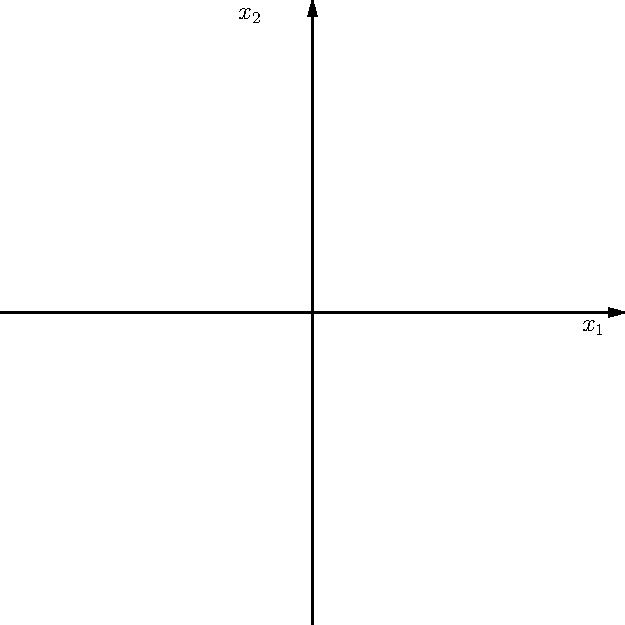
\includegraphics[width=.6\textwidth{}]{coord.pdf}
  \end{figure}
\end{frame}

\begin{frame}{约束的几何表示}
  \begin{figure}[b]
    \centering
    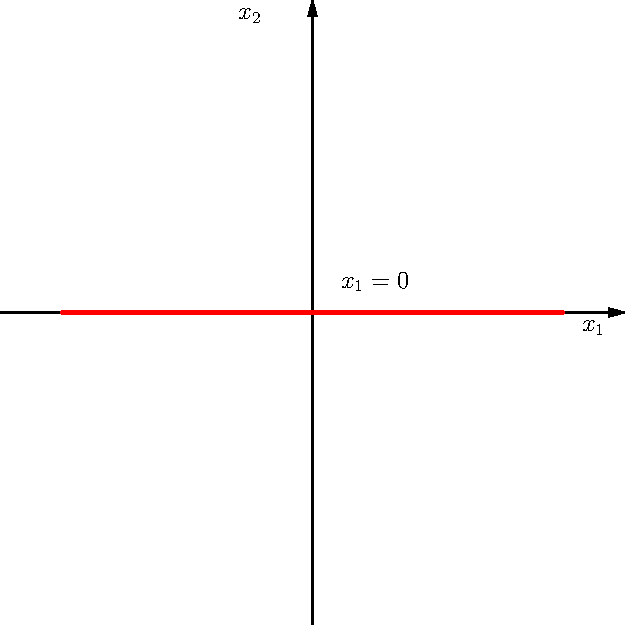
\includegraphics[width=.6\textwidth{}]{equal.pdf}
  \end{figure}
\end{frame}

\begin{frame}{约束的几何表示}
  \begin{figure}[b]
    \centering
    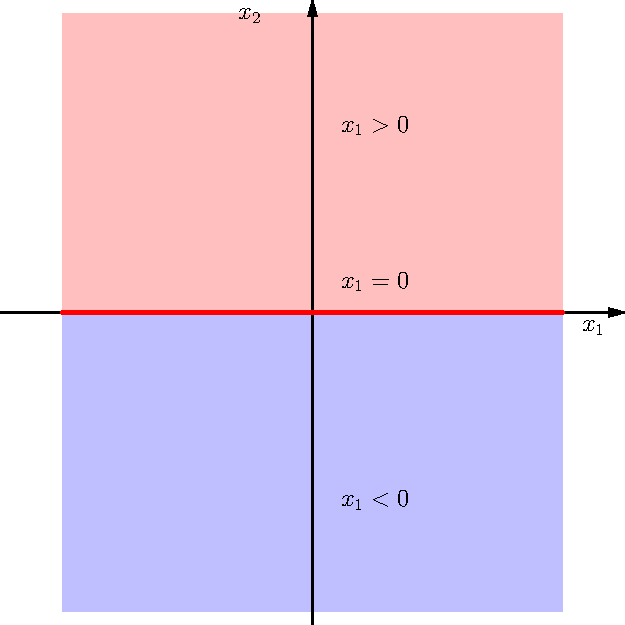
\includegraphics[width=.6\textwidth{}]{halfplane.pdf}
  \end{figure}  
\end{frame}

\begin{frame}{约束的几何表示}
  \[
  \begin{array}{l}
    x_1 + 2x_2 \le 4\\
    x1, x2 \ge 0
  \end{array}
  \]
  \begin{figure}
    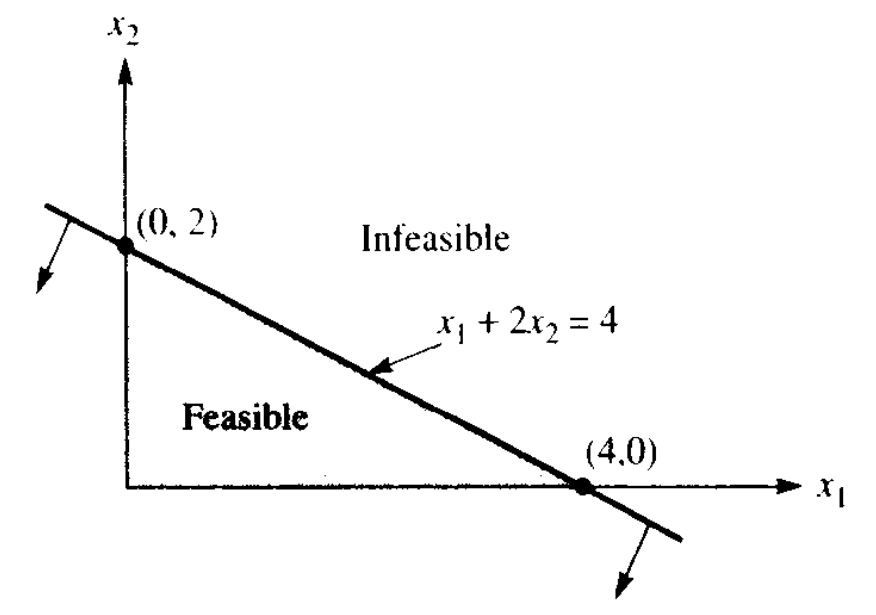
\includegraphics[width=.5\textwidth{}]{feasible.png}
    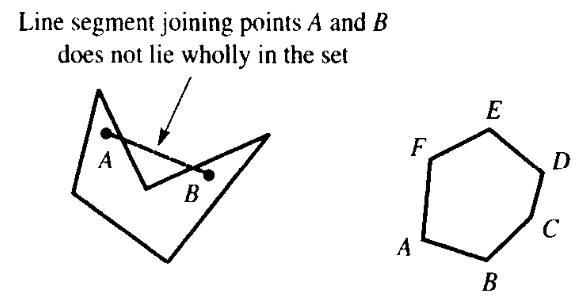
\includegraphics[width=.5\textwidth{}]{convex.png}
  \end{figure}  

  \begin{itemize}
  \item 满足条件的所有点构成一个凸集
  \item 最优解是凸集的一个角点
  \end{itemize}

\end{frame}

\begin{frame}{木匠问题}
  \begin{figure}
    \begin{minipage}{.5\linewidth}
      \[ 
      \begin{array}{lcl}
        & \mbox{Max}\ 25x_1 + 30x_2 & \\
        \mbox{s.t.} & &  \\
        &
        \begin{array}{c}
          20x_1 + 30x_2 \le 690 (\text{木板})\\
          5x_1 + 4x_2 \le 120 (\text{劳动时间})\\
          x_1, x_2 \ge 0 (\text{非负性})
        \end{array}
        &
      \end{array}
      \]
    \end{minipage}%
    \begin{minipage}{.5\linewidth}
      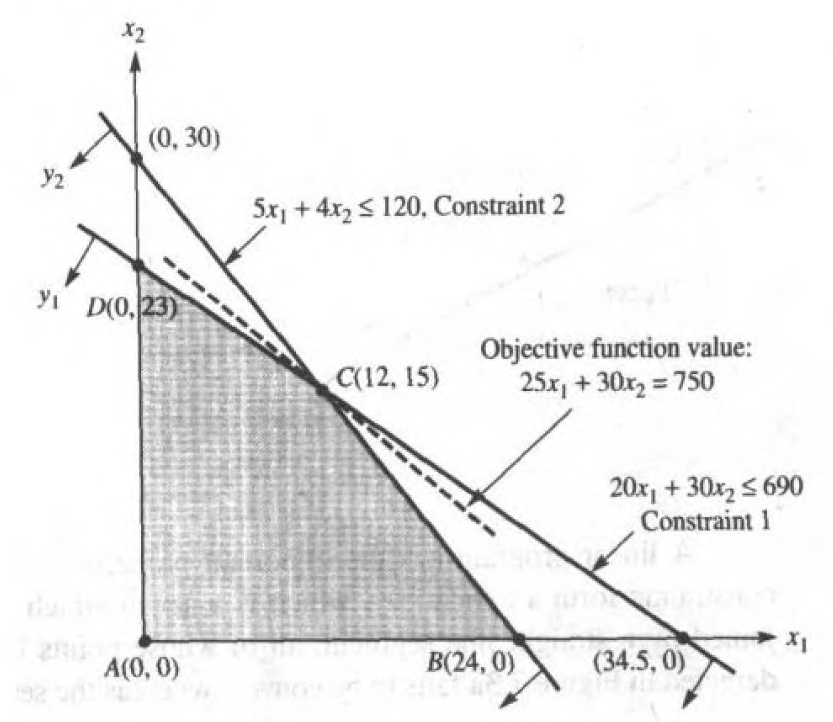
\includegraphics[width=\textwidth{}]{wood.png}    
    \end{minipage}
  \end{figure}
  \begin{table}
    \centering
    \begin{tabular}{lc}
      极点 & 目标函数值(美元)\\[-5pt]
      $A(0, 0)$ & 0 \\[-5pt]
      $B(24, 0)$ & 600 \\[-5pt]
      $C(12, 15)$ & 750 \\[-5pt]
      $D(0, 23)$ & 690
    \end{tabular}
  \end{table}
  
\end{frame}

\begin{frame}{数据拟合问题}
  用切比雪夫准则拟合模型$y=cx$:\quad{}
  \begin{tabular}{c|ccc}
    x & 1 & 2 & 3\\
    \hline\\[-20pt]
    y & 2 & 5 & 8
  \end{tabular}

  \begin{figure}
    \begin{minipage}{.5\linewidth}
    \[ 
    \begin{array}{c}
      \mbox{Min}\ r\\
      \begin{array}{ll}
        \mbox{s.t.} & \\
        &
        \begin{array}{r}
          r - (2 - c) \ge 0 \\
          r + (2 - c) \ge 0 \\
          r - (5 -2c) \ge 0 \\
          r + (5 - 2c) \ge 0 \\
          r - (8 - 3c) \ge 0 \\
          r + (8 - 3c) \ge 0
        \end{array}
      \end{array}
    \end{array}
    \]
    \end{minipage}%
    \begin{minipage}{.5\linewidth}
      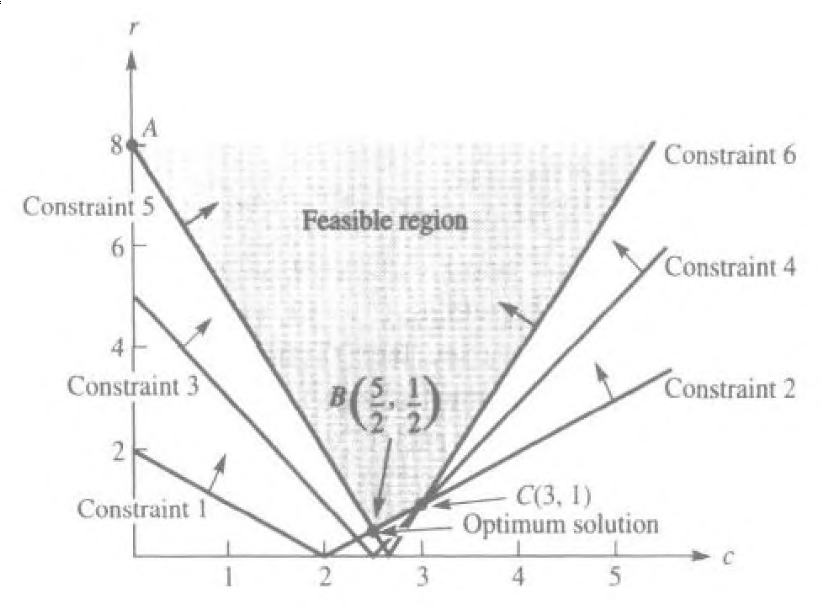
\includegraphics[width=\textwidth{}]{datafit.png}
    \end{minipage}
  \end{figure}
  
  $r_{max} = \frac{1}{2}$(B点)
  
\end{frame}

\begin{frame}{可行域}
  \begin{itemize}
  \item 空可行域
    \[
    \left\{
    \begin{array}{l}
      x_1 \le 3\\
      x_1 \ge 5
    \end{array}
    \right.
    \]
  \item 无界可行域
    \[
    \mbox{Max}\ x_1 + x_2
    \]
  \end{itemize}
\end{frame}

\begin{frame}{目标函数的等值曲线}
  \begin{figure}
      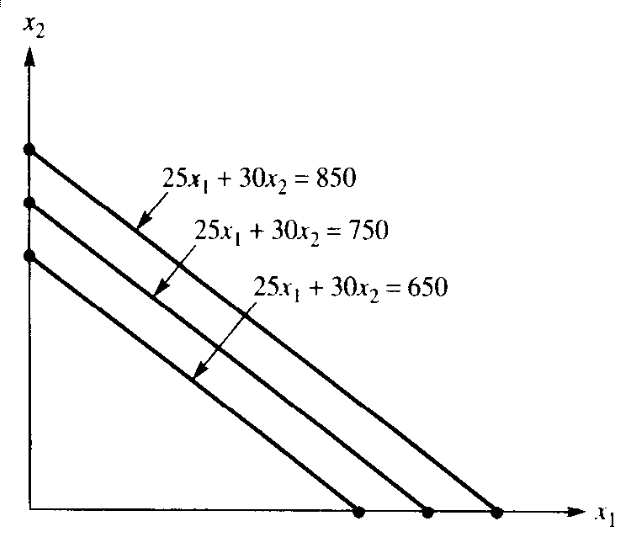
\includegraphics[width=.4\textwidth{}]{level.png}
      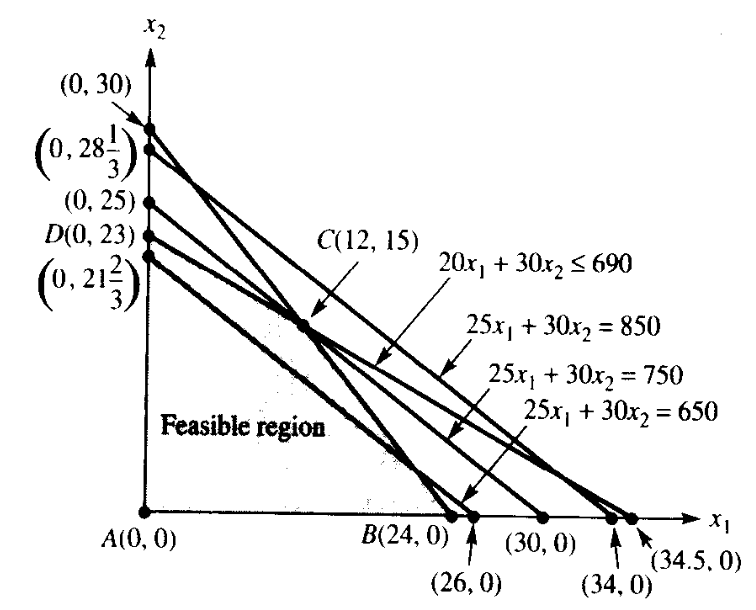
\includegraphics[width=.5\textwidth{}]{levelcons.png}
  \end{figure}
\end{frame}

\begin{frame}{约束函数与目标函数平行}
  \begin{figure}
    \begin{minipage}{.5\linewidth}
      \[ 
      \begin{array}{lcl}
        & \mbox{Max}\ 25x_1 + 30x_2 & \\
        \mbox{s.t.} & &  \\
        &
        \begin{array}{c}
          25x_1 + 30x_2 \le 690 (\text{木板})\\
          5x_1 + 4x_2 \le 150 (\text{劳动时间})\\
          x_1, x_2 \ge 0 (\text{非负性})
        \end{array}
        &
      \end{array}
      \]
    \end{minipage}%
    \begin{minipage}{.5\linewidth}
      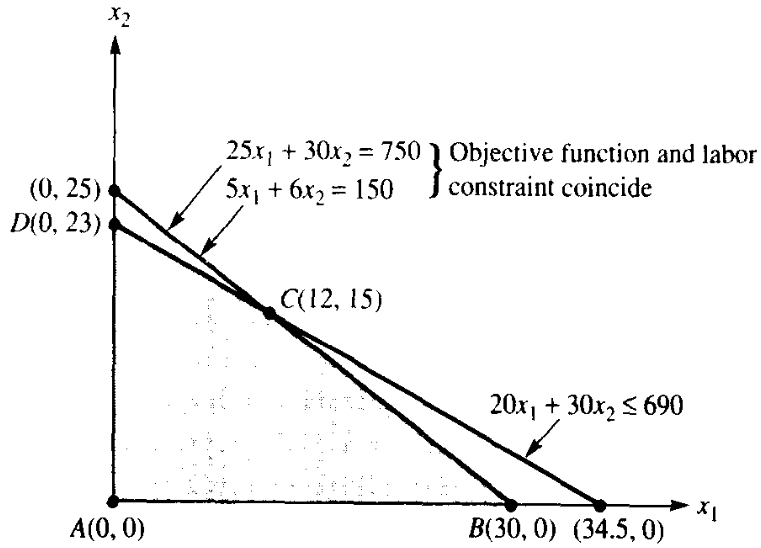
\includegraphics[width=\textwidth{}]{coincide.png}
    \end{minipage}
  \end{figure}

  无穷多个最优解

\end{frame}

\begin{frame}{几何法总结}
  \begin{block}{定理1}
    假设线性规划的可行域是非空有界凸集,则目标函数一定会在可行域的极点上取到最大值和最小值。如果可行域无界,目标函数不一定能取到最优值;然而,如果最大值和最小值确实存在,则一定会在某个极点上取到
  \end{block}

  \begin{figure}
    \centering
    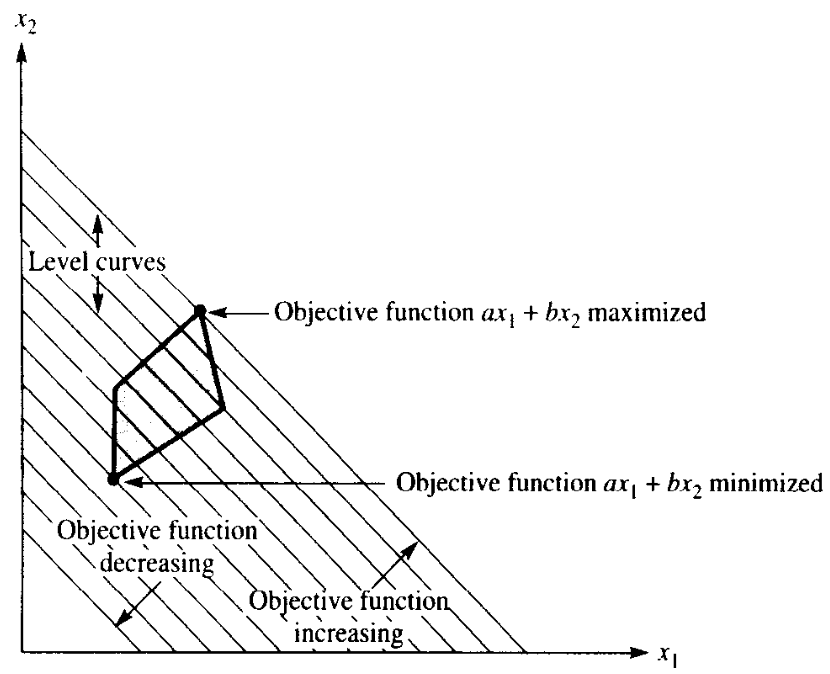
\includegraphics[width=.4\textwidth{}]{extreme.png}
  \end{figure}
\end{frame}

\begin{frame}{代数解法}
  木匠问题的图解法提出了在非空有界可行域上求线性规划问题最优解的基本步骤:
  \begin{enumerate}
  \item 找到约束的所有交点
  \item 判断哪个交点是可行解(如果有的话),从而得到所有极点
  \item 计算每个极点的目标函数值
  \item 选择使目标函数值取到最大(最小)的极点
  \end{enumerate}
  
\end{frame}

\begin{frame}{代数解法}
  \begin{figure}
    \centering
    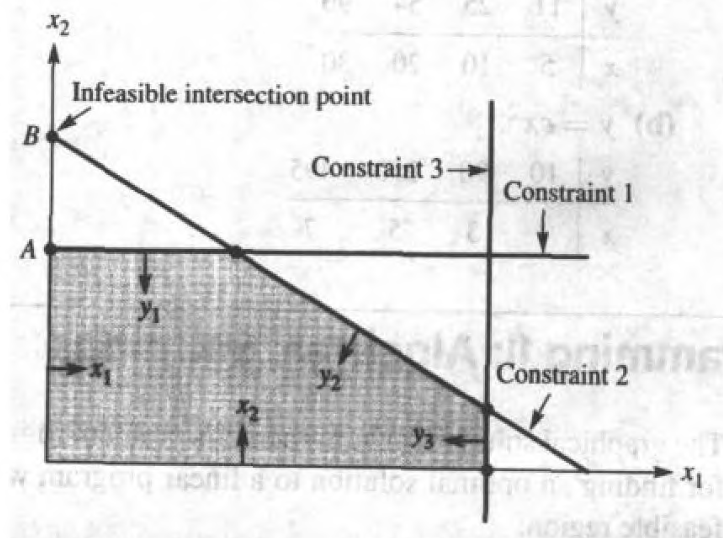
\includegraphics[width=.6\textwidth{}]{inter.png}
  \end{figure}

  \begin{itemize}
  \item 变量$y_1$, $y_2$, $y_3$表示一个点满足约束1,2,3的程度
  \item 考虑变量$\{x_1, x_2, y_1, y_2, y_3\}$
    \begin{itemize}
    \item 一个为0,表示点在边界上
    \item 两个为0,表示一个交点
    \end{itemize}
  \end{itemize}
\end{frame}

\begin{frame}{木匠问题的代数解法}
  \begin{figure}
    \begin{minipage}{.5\linewidth}
      \[ 
      \begin{array}{lcl}
        & \mbox{Max}\ 25x_1 + 30x_2 & \\
        \mbox{s.t.} & &  \\
        &
        \begin{array}{c}
          20x_1 + 30x_2 + y_1 = 690\\
          5x_1 + 4x_2 + y_2 = 120\\
          x_1, x_2, y_1, y_2 \ge 0
        \end{array}
        &
      \end{array}
      \]
    \end{minipage}%
    \begin{minipage}{.5\linewidth}
      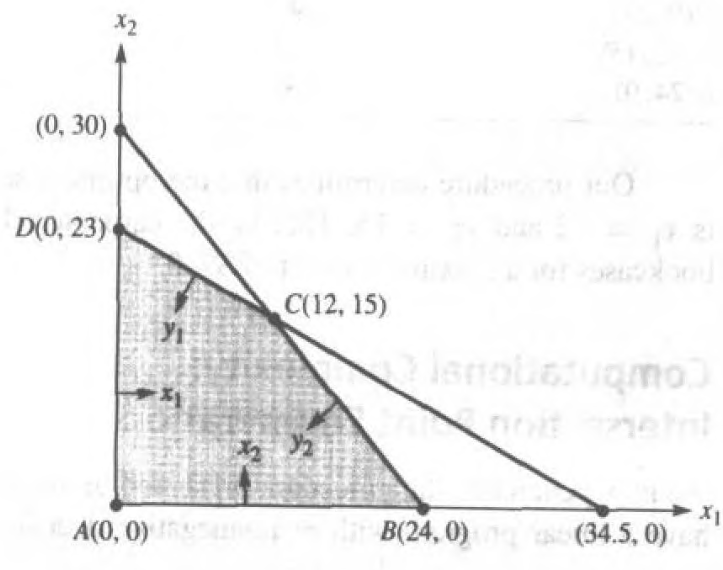
\includegraphics[width=\textwidth{}]{wood-var.png}
    \end{minipage}
  \end{figure}
  
  \begin{itemize}
  \item 四个变量$\{x_1, x_2, y_1, y_2\}$,其中两个为0表示一个交点,共$4!/(2!2!)=6$种情况
  \item 通过方程可解出另外两个变量的值,若都大于0,则是一个可行解
  \item 找出可行解中使得目标函数最大的,即是最优解
  \end{itemize}

\end{frame}

\begin{frame}{木匠问题的代数解法}
  \begin{itemize}
  \item 令$x_1 = x_2 = 0$, 解出$y_1 = 690, y_2 = 120$,得到交点$A(0,0)$是可行解,目标函数值0
  \item 令$x_1 = y_1 = 0$, 解出$x_2 = 23, y_2 = 28$,得到交点$D(0,23)$是可行解,目标函数值690
  \item 令$x_1 = y_2 = 0$, 解出$x_2 = 30, y_1 = -210$,不是可行解
  \item 令$y_1 = y_2 = 0$, 解出$x_1 = 12, x_2 = 15$,得到交点$C(12,15)$是可行解,目标函数值750
  \item 令$x_2 = y_1 = 0$, 解出$x_1 = 34.5, y_2 = -52.5$,不是可行解
  \item 令$x_2 = y_2 = 0$, 解出$x_1 = 24, y_1 = 210$,得到交点$B(24,0)$是可行解,目标函数值600
  \end{itemize}
  
\end{frame}

\begin{frame}{枚举交点的计算复杂性}

  假定一个线性规划有$m$个非负决策变量和$n$个约束,其中每个约束都是$\le$的形式.
  \begin{itemize}
  \item 对第$i$个约束增加新的非负``松弛''变量$y_i$,将每个不等式转化为等式
  \item 总共有$m+n$的非负变量,为了确定一个交点,从中选择$m$个变量(因为有$m$个决策变量)并令其为0,一共有$(m+n)!/(m!n!)$个可能的选择需要考虑.
  \item 当线性规划的规模增加是计算量急剧增加
  \end{itemize}
  
\end{frame}

\begin{frame}{如何减少计算量?}

  \begin{itemize}
  \item 如何快速判断一个可能的交点是不可行的?
  \item 找到一个极点并知道其目标函数值,能否快速判定另一个极点是否能够进一步对目标函数值有所改进?
  \end{itemize}

  单纯形法!
  
\end{frame}

\begin{frame}{单纯形法}
  \begin{block}{}
    George Dantzig发明的单纯形法,融合了最优性检验和可行性检验,从而找到线性规划问题的最优解(如果最优解存在的话)
  \end{block}

  \begin{description}
  \item[最优性检验] 判断一个交点对应的目标函数值是否比当前找到的最好结果更优
  \item[可行性检验] 判断一个交点是否可行
  \end{description}

\end{frame}

\begin{frame}{单纯形法的步骤}
  首先将决策变量和松弛变量分成两个互不相交的集合,即独立变量集合和相关变量集合。

  \begin{block}{步骤}
    \begin{enumerate}
    \item 表格形式:将线性规划放在表格形式中
    \item 初始极点:单纯形法从一个已知的极点开始,通常为原点$(0,0)$
    \item 最优性检验:判断与当前极点相邻的交点是能否改进目标函数值
    \item 可行性检验:为找到一个可行的新交点,选择一个相关变量退出
    \item 旋转:令新的独立变量为0,解出相关变量,确定一个交点
    \item 重复步骤$3 - 5$,直到找到一个最优的极点
    \end{enumerate}
  \end{block}

\end{frame}

\begin{frame}{木匠问题}
  \begin{figure}
    \begin{minipage}{.5\linewidth}
      \[ 
      \begin{array}{lcl}
        & \mbox{Max}\ 25x_1 + 30x_2 & \\
        \mbox{s.t.} & &  \\
        &
        \begin{array}{c}
          20x_1 + 30x_2 \le 690 (\text{木板})\\
          5x_1 + 4x_2 \le 120 (\text{劳动时间})\\
          x_1, x_2 \ge 0 (\text{非负性})
        \end{array}
        &
      \end{array}
      \]
    \end{minipage}%
    \begin{minipage}{.5\linewidth}
      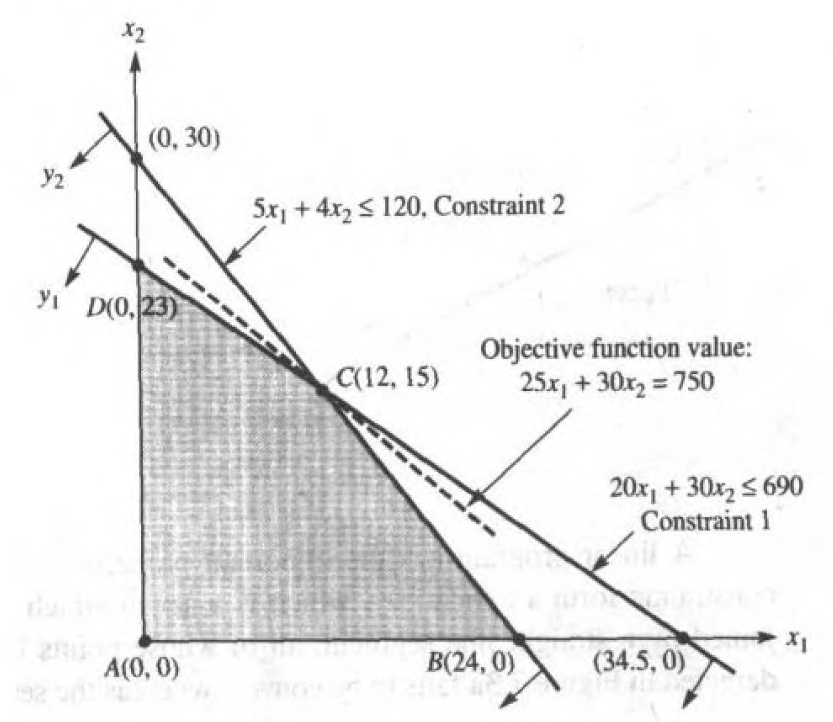
\includegraphics[width=\textwidth{}]{wood.png}    
    \end{minipage}
  \end{figure}

  \begin{block}{}
    从几何上看,单纯形法是从一个初始极点移动到一个相邻的极点,直到没有更优的相邻极点。这时,当前的极点就是最优解。
  \end{block}
\end{frame}

\begin{frame}{第1步 构造单纯形表}
  假定问题是最大化目标函数,并且约束条件是用小于等于形式的不等式表示的(如果初始问题不是这种形式,很容易将它变成这种形式)。

  \[ 
  \begin{array}{lcl}
    & \mbox{Max}\ 25x_1 + 30x_2 & \\
    \mbox{s.t.} & &  \\
    &
    \begin{array}{c}
      20x_1 + 30x_2 \le 690 (\text{木板})\\
      5x_1 + 4x_2 \le 120 (\text{劳动时间})\\
      x_1, x_2 \ge 0 (\text{非负性})
    \end{array}
    &
  \end{array}
  \]

  增加一个新的约束,使得目标函数值优于当前值:

  \[
  25x_1 + 30x_2 \ge 0 \Longrightarrow -25x_1 - 30x_2 \le 0
  \]

  单纯形法隐含地假定所有的变量都非负

\end{frame}

\begin{frame}{第1步 构造单纯形表}
  通过增加新的非负变量,将不等式约束转化为等式约束

  \[
    \begin{array}{c}
      20x_1 + 30x_2 + y_1 = 690\\
      5x_1 + 4x_2 + y_2 =  120\\
      -25x_1 - 30x_2 + z = 0
    \end{array}
  \]

  其中$x_1, x_2, y_1, y_2$非负,变量$z$表示的是目标函数值。

\end{frame}

\begin{frame}{第2步 选取初始极点}

  \begin{figure}
    \begin{minipage}{.5\linewidth}
      \begin{itemize}
      \item 有两个决策变量
      \item 通过将$\{x_1, x_2, y_1, y_2\}$中的某两个变量设为0可以得到一个交点
      \item $z$总是相关变量,表示目标函数的值
      \item 原点是一个可行点,对应$x_1=x_2=0, y_1=690, y_2=120$,此时$x_1, x_2$是独立变量,$y_1, y_2, z$是相关变量
      \end{itemize}
    \end{minipage}%
    \begin{minipage}{.5\linewidth}
      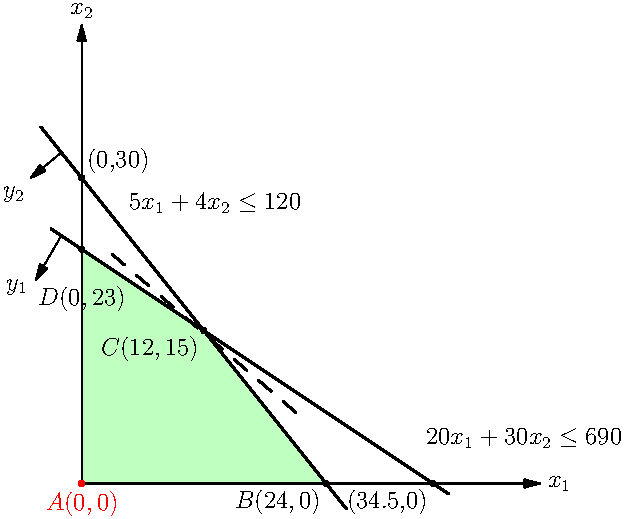
\includegraphics[width=\textwidth{}]{simplex-init.pdf}
    \end{minipage}
  \end{figure}

  
\end{frame}

\begin{frame}{第3步 最优性检验选择进入变量}
  \begin{figure}
    \begin{minipage}{.5\linewidth}
      \begin{itemize}
      \item 最后的等式中若有负的系数,则该变量成为相关变量会改进目标函数
      \item 若有多变量可选,选择系数绝对值最大的
      \item 如果不存在负系数,则已取得最优值
      \end{itemize}
    \end{minipage}%
    \begin{minipage}{.5\linewidth}
      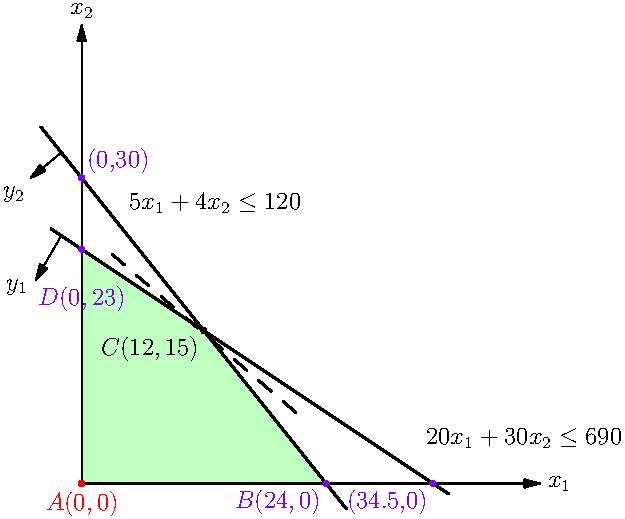
\includegraphics[width=\textwidth{}]{simplex-improve.pdf}
    \end{minipage}
  \end{figure}  
\end{frame}

\begin{frame}{第4步 可行性检验选择退出变量}
  \begin{figure}
    \begin{minipage}{.5\linewidth}
      \begin{itemize}
      \item 需确定进入的变量到底是$y_1$还是$y_2$
      \item 用原约束右边的项除以即将退出的变量的系数,即分别690/30=23, 120/4=30
      \item 从取正数的比值中选择较小的对应变量退出(即$y_1$,对应23)
      \item 含义:如果对应变量退出相关变量并被赋0后,新进入变量的取值
      \end{itemize}
    \end{minipage}%
    \begin{minipage}{.5\linewidth}
      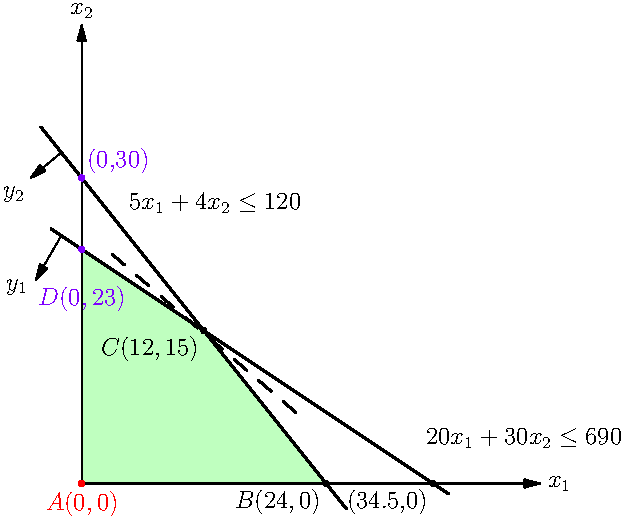
\includegraphics[width=\textwidth{}]{simplex-feasible.pdf}
    \end{minipage}
  \end{figure}  
\end{frame}

\begin{frame}{第5步 通过旋转计算新的相关变量的取值}
  \begin{figure}
    \begin{minipage}{.5\linewidth}
      \begin{itemize}
      \item 通过消元法使得每个约束方程只含有一个相关变量
      \item 然后继续执行第3步
      \end{itemize}
    \end{minipage}%
    \begin{minipage}{.5\linewidth}
      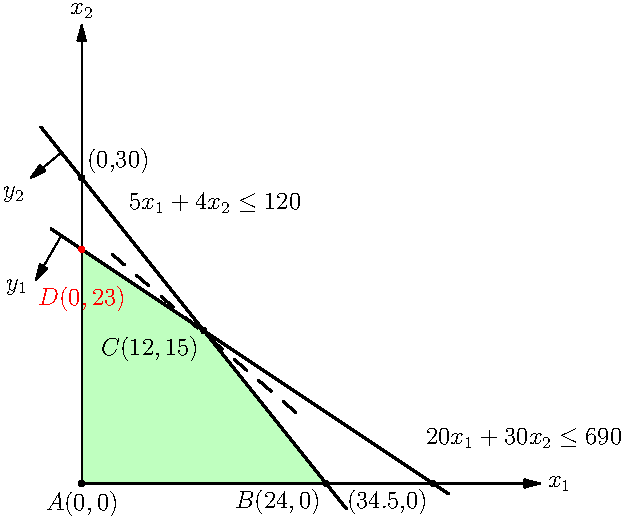
\includegraphics[width=\textwidth{}]{simplex-rotate.pdf}
    \end{minipage}
  \end{figure}  
\end{frame}

\begin{frame}{单纯形方法的总结}
  \begin{enumerate}
  \item 将问题至于表格形式中,如果有需要,增加松弛变量,将不等式约束转化成等式。请记住,所有变量都是非负的。将目标函数约束作为最后一个约束,包括它对于的松弛变量$z$
  \item 找到一个初始点(通常是原点)
  \item 进行最优性检验。检查最后一个方程(对于目标函数),如果所有系数非负,则停机,当前的极点最优;否则,有些变量系数为负,选择其中绝对值最大的,作为新的进入变量。
  \item 进行可行性检验。用右端项除以进入变量系数,选择最小的正比值对于变量退出。
  \item 旋转。通过消元法使得每个约束方程只含有一个相关变量
  \end{enumerate}
\end{frame}

\begin{frame}{再论木匠问题}
  \begin{description}
  \item[第1步] 表格形式为:
    \[
    \begin{array}{c}
      20x_1 + 30x_2 + y_1 = 690\\
      5x_1 + 4x_2 + y_2 =  120\\
      -25x_1 - 30x_2 + z = 0
    \end{array}
    \]
  \item[第2步] 原点$(0,0)$是一个初始极点,独立变量是$x_1=x_2=0$,相关变量是$y_1=690, y_2=120, z=0$
  \item[第3步] 进行最优性检验,选取$x_2$为进行相关变量集合的变量,因为它对应于绝对值最大的负系数。
  \item[第4步] 进行可行性检验,用右端项的690和120,除以进入变量$x_2$在每个方程中对应的系数(分别为30和4),得到比值23和30,最小比值为23,对应与第一个方程,松弛变量是$y_1$,所以选它作为退出变量。
  \end{description}

\end{frame}

\begin{frame}{再论木匠问题}
  \begin{description}
  \item[第5步] 通过旋转,令独立变量$x_1$, $y_1$的取值为0,找出新相关变量$x_2, y_2, z$的取值。从不包含退出变量$y_1$的方程中,消去新的相关变量$x_2$,得到等价方程组:
    \[
    \begin{array}{c}
      \frac{2}{3}x_1 + x_2 + \frac{1}{30}y_1 = 23\\
      \frac{7}{3}x_1 - \frac{2}{15}y_1 + y_2 =  28\\
      -5x_1 + y_1 + z = 690
    \end{array}
    \]
    令$x_1=y_1=0$,得到$x_2=23, y_2=28,z=690$.结果,得到极点(0,23),目标函数值$z=690$
  \end{description}
  
\end{frame}

\begin{frame}{表格法 - 最优性检验}

  \begin{table}
    \centering
    \begin{tabular}{|ccccc|c|}
      \hline
      $x_1$ & {\color{red}$x_2$} & $y_1$ & $y_2$ & $z$ & 右端项 \\
      \hline
      20 & 30 & 1 & 0 & 0 & 690(=$y_1$)\\
      5 & 4 & 0 & 1 & 0 & 120(=$y_2$)\\
      \hline
      -25 & {\color{red} -30} & 0 & 0 & 1 & 0(=$z$)\\
      \hline
    \end{tabular}
    \caption{单纯形表0(原始表)}
  \end{table}

  \begin{description}
  \item[相关变量] $\{y_1, y_2, z\}$
  \item[独立变量] $x_1=x_2=0$
  \item[极点] $(x_1, x_2) = (0, 0)$
  \item[目标函数值] $z = 0$
  \end{description}

\end{frame}

\begin{frame}{表格法 - 可行性检验}

  \begin{table}
    \centering
    \begin{tabular}{|ccccc|c|c|}
      \hline
      $x_1$ & {\color{red} $x_2$} & $y_1$ & $y_2$ & $z$ & 右端项 & 比值 \\
      \hline
      20 & 30 & 1 & 0 & 0 & 690 & {\color{green}23(=690/30)}\\
      5 & 4 & 0 & 1 & 0 & 120 & 30(=120/4)\\
      \hline
      -25 & {\color{red} -30} & 0 & 0 & 1 & 0 &*\\
      \hline
    \end{tabular}
  \end{table}

  \begin{description}
  \item[相关变量] $\{y_1, y_2, z\}$
  \item[独立变量] $x_1=x_2=0$
  \item[极点] $(x_1, x_2) = (0, 0)$
  \item[目标函数值] $z = 0$
  \end{description}

\end{frame}

\begin{frame}{表格法 - 最优性检验}

  \begin{table}
    \centering
    \begin{tabular}{|ccccc|c|}
      \hline
      {\color{red}$x_1$} & $x_2$ & $y_1$ & $y_2$ & $z$ & 右端项 \\
      \hline
      0.66667 & 1 & 0.03333 & 0 & 0 & 23(=$x_2$)\\
      2.33333 & 0 & -0.13333 & 1 & 0 & 28(=$y_2$)\\
      \hline
      {\color{red}-5} & 0 & 1 & 0 & 1 & 690(=$z$)\\
      \hline
    \end{tabular}
    \caption{单纯形表1}
  \end{table}

  \begin{description}
  \item[相关变量] $\{x_2, y_2, z\}$
  \item[独立变量] $x_1=y_1=0$
  \item[极点] $(x_1, x_2) = (0, 23)$
  \item[目标函数值] $z = 690$
  \end{description}

\end{frame}

\begin{frame}{表格法 - 可行性检验}

  \begin{table}
    \centering
    \begin{tabular}{|ccccc|c|c|}
      \hline
      {\color{red}$x_1$} & $x_2$ & $y_1$ & $y_2$ & $z$ & 右端项 & 比值\\
      \hline
      0.66667 & 1 & 0.03333 & 0 & 0 & 23 & 34.5(=23/0.66667)\\
      2.33333 & 0 & -0.13333 & 1 & 0 & 28 & {\color{green}12.0(=28/2.33333)}\\
      \hline
      {\color{red}-5} & 0 & 1 & 0 & 1 & 690 & *\\
      \hline
    \end{tabular}
  \end{table}

  \begin{description}
  \item[相关变量] $\{x_2, y_2, z\}$
  \item[独立变量] $x_1=y_1=0$
  \item[极点] $(x_1, x_2) = (0, 23)$
  \item[目标函数值] $z = 690$
  \end{description}

\end{frame}

\begin{frame}{表格法 - 最优性检验}

  \begin{table}
    \centering
    \begin{tabular}{|ccccc|c|}
      \hline
      $x_1$ & $x_2$ & $y_1$ & $y_2$ & $z$ & 右端项 \\
      \hline
      0 & 1 & 0.071429 & -0.28571 & 0 & 15(=$x_2$)\\
      1 & 0 & -0.057143 & 0.42857 & 0 & 12(=$x_1$)\\
      \hline
      0 & 0 & 1 & 0.714286 & 2.14286 & {\color{green}750(=$z$)}\\
      \hline
    \end{tabular}
    \caption{单纯形表2}
  \end{table}

  \begin{description}
  \item[相关变量] $\{x_1, x_2, z\}$
  \item[独立变量] $y_1=y_2=0$
  \item[极点] $(x_1, x_2) = (12, 15)$
  \item[目标函数值] $z = 750$
  \end{description}

\end{frame}

\begin{frame}{敏感性分析}
  \begin{itemize}
  \item 每张桌子的利润在什么范围内取值时,当前最优解仍然是最优的?
  \item 劳动时间增加一个单位时,价值有多大?
  \end{itemize}
  \[
  \mbox{Max}\ 25x_1 + 30x_2
  \]

  \begin{figure}
    \begin{minipage}{.5\linewidth}
      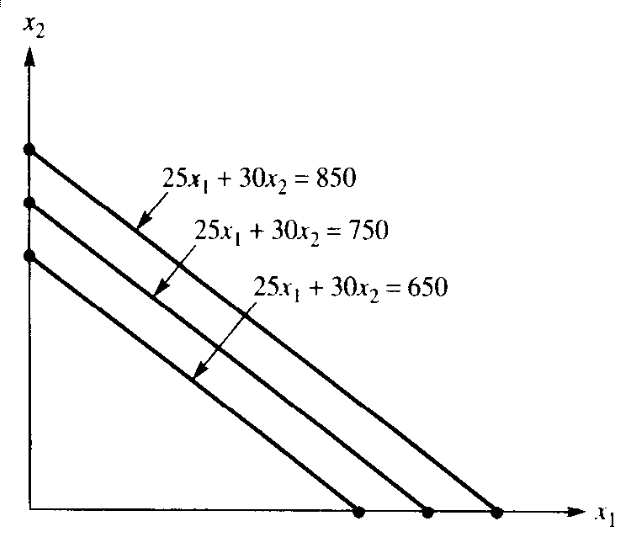
\includegraphics[width=\textwidth{}]{level.png}
    \end{minipage}%
    \begin{minipage}{.5\linewidth}
      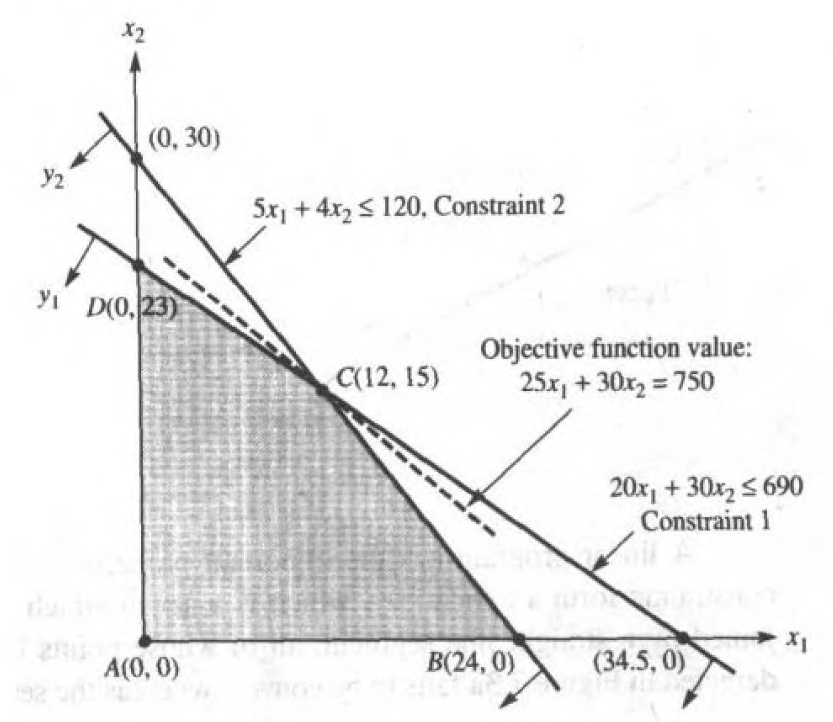
\includegraphics[width=\textwidth{}]{wood.png}
    \end{minipage}
  \end{figure}  

\end{frame}

\begin{frame}{改变每张桌子的利润$c_1$}
  \[
  \mbox{Max}\ c_1x_1 + 30x_2
  \]

  \begin{figure}
    \begin{minipage}{.5\linewidth}
      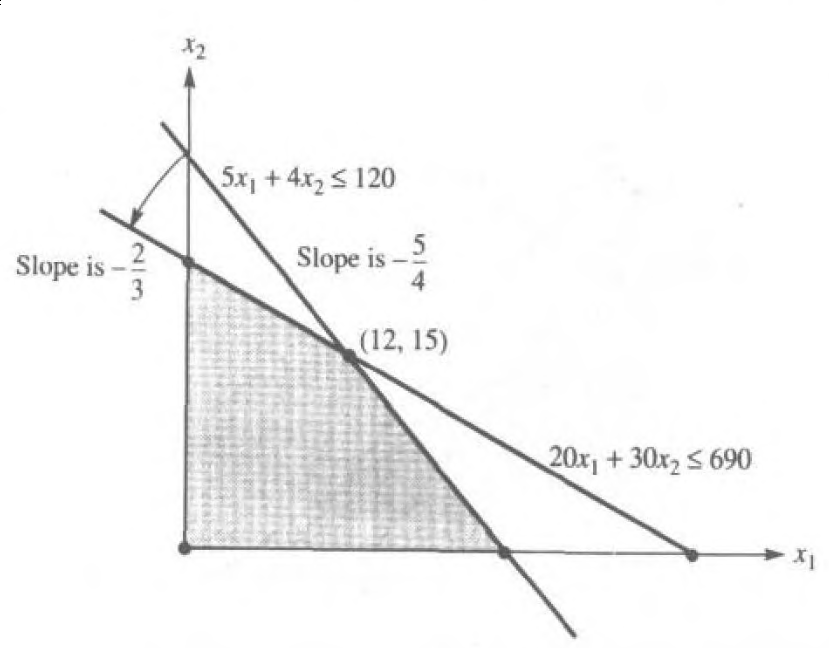
\includegraphics[width=\textwidth{}]{table.png}
    \end{minipage}%
    \begin{minipage}{.5\linewidth}
      \[
      -\frac{5}{4} \le -\frac{c_1}{30} \le -\frac{2}{3}
      \]

      即
      \[
      20 \le c_1 \le 37.5
      \]

    \end{minipage}
  \end{figure}  

\end{frame}

\begin{frame}{可利用资源的变化}
  劳动时间的变化:
  \[
  5x_1 + 4x_2 \le b_2
  \]

  \begin{figure}
    \begin{minipage}{.5\linewidth}
      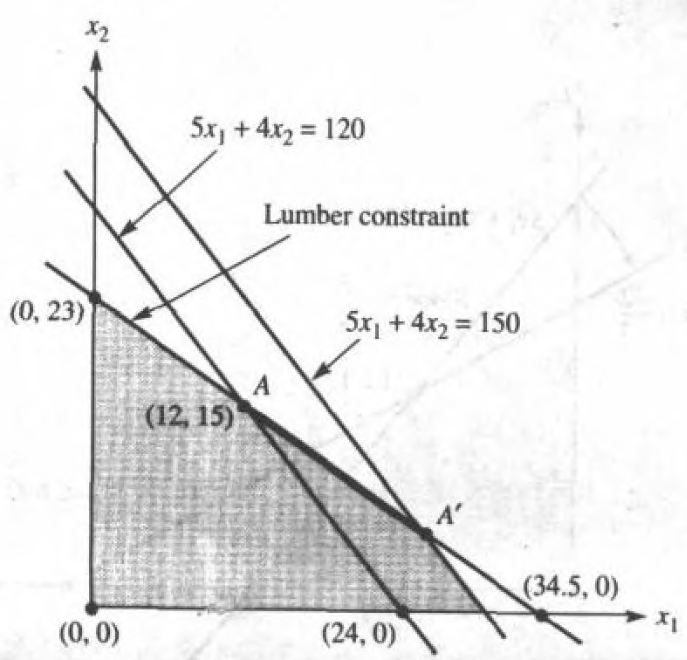
\includegraphics[width=\textwidth{}]{labor.png}
    \end{minipage}%
    \begin{minipage}{.5\linewidth}
      只要$b_2$在下面的范围内,最优解将沿着木板约束移动:
      \[
      92 \le b_2 \le 172.5
      \]
    \end{minipage}
  \end{figure}  

\end{frame}

\begin{frame}{可利用资源的变化}
  劳动时间的变化:
  \[
  5x_1 + 4x_2 \le b_2
  \]

  \begin{figure}
    \begin{minipage}{.5\linewidth}
      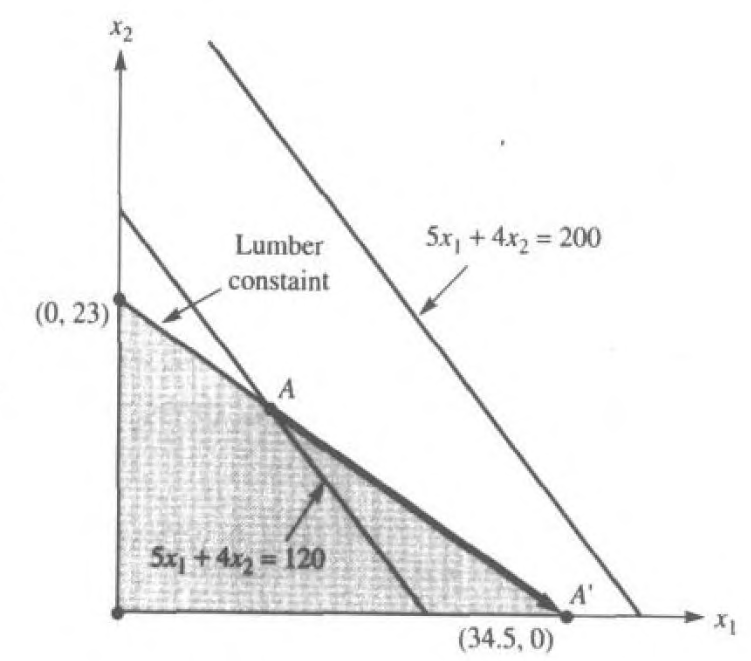
\includegraphics[width=\textwidth{}]{labor2.png}
    \end{minipage}%
    \begin{minipage}{.5\linewidth}
      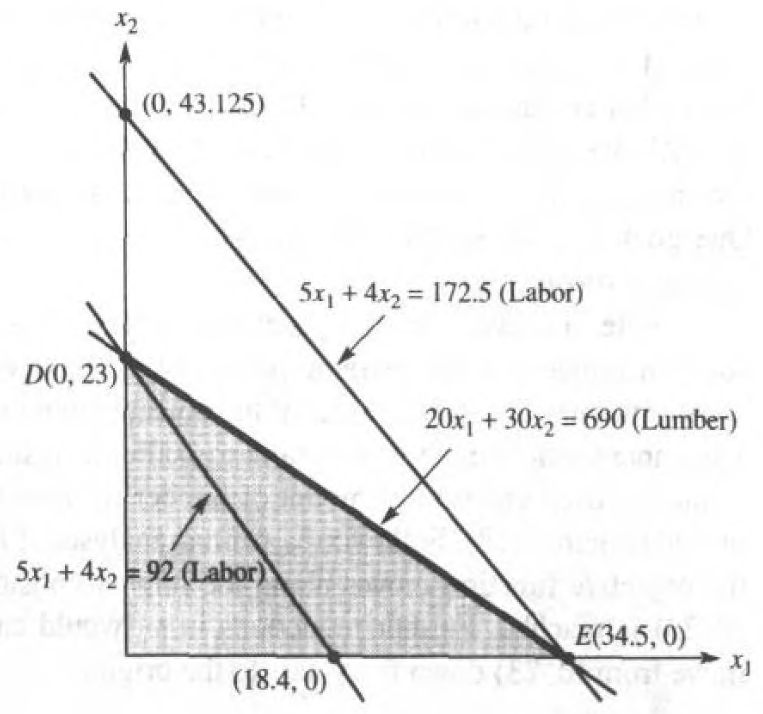
\includegraphics[width=\textwidth{}]{labor3.png}
    \end{minipage}
  \end{figure}  

\end{frame}

\begin{frame}{Matlab中的线性规划函数}
  \begin{figure}
    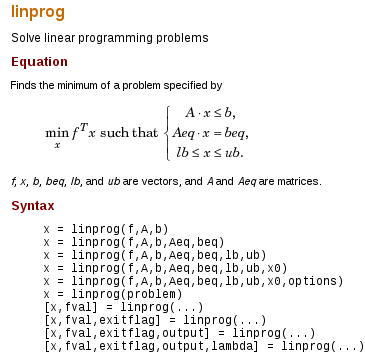
\includegraphics[height=\textheight{}]{linprog.png}
  \end{figure}  

\end{frame}

\begin{frame}{数值搜索方法}
  \begin{itemize}
  \item 假设函数$f(x)$在区间$[a,b]$是单峰的,求其极值点$x^*$
  \end{itemize}

  \begin{figure}
    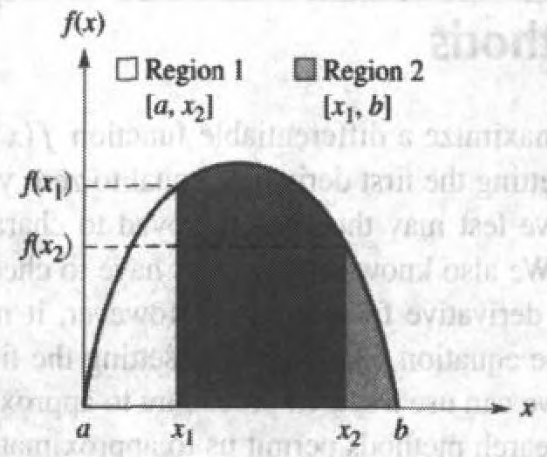
\includegraphics[width=.4\textwidth{}]{part.png}

    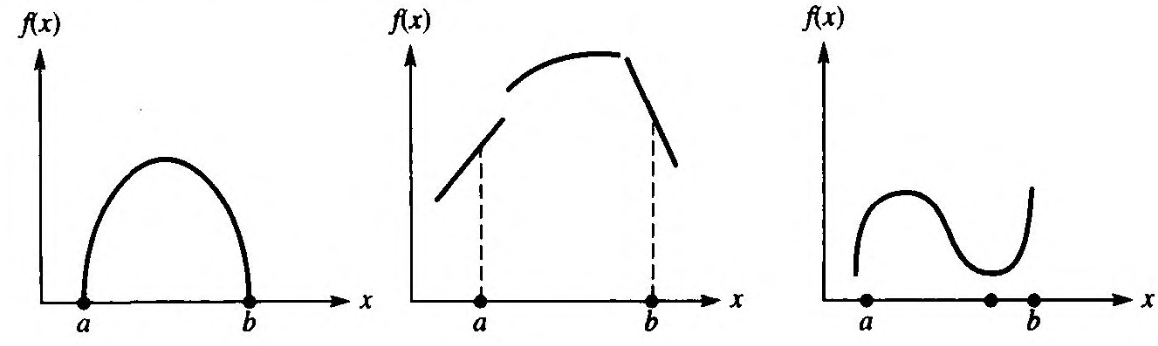
\includegraphics[width=.8\textwidth{}]{unimodal.png}
  \end{figure}  
  
\end{frame}

\begin{frame}{搜索方法概貌}
  \begin{description}
  \item[情形1] $f(x_1) < f(x_2)$. 因为$f(x)$是单峰的,最优解不能位于区间$[a, x_1]$,只能位于$(x_1, b]$.
  \item[情形2] $f(x_1) > f(x_2)$. 因为$f(x)$是单峰的,最优解不能位于区间$[x_2, b]$,只能位于$[a, x_2]$.
  \item[情形3] $f(x_1) = f(x_2)$. 最优解只能位于$(x_1, x_2)$.
  \end{description}

  \begin{figure}
    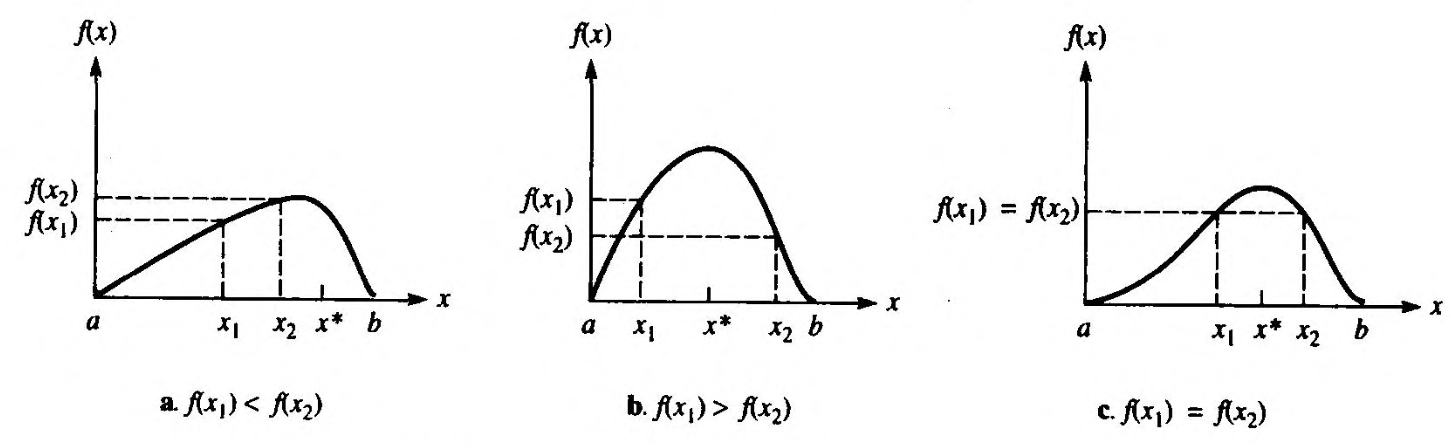
\includegraphics[width=\textwidth{}]{search.png}
  \end{figure}  

\end{frame}

\begin{frame}{二分搜索}
  \begin{figure}
    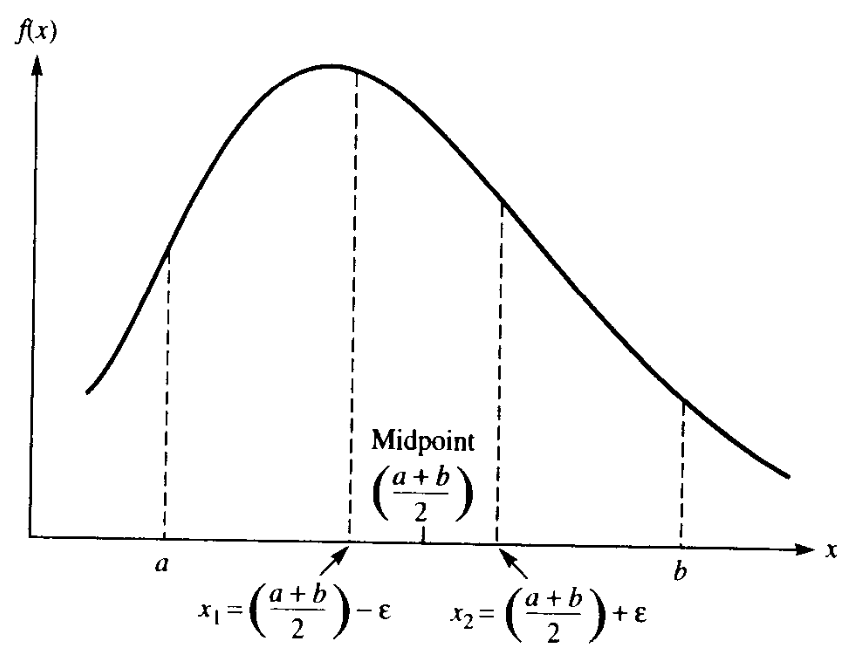
\includegraphics[height=.8\textheight{}]{binary.png}
  \end{figure}    
\end{frame}

\begin{frame}{黄金分隔搜索}
  \begin{figure}
    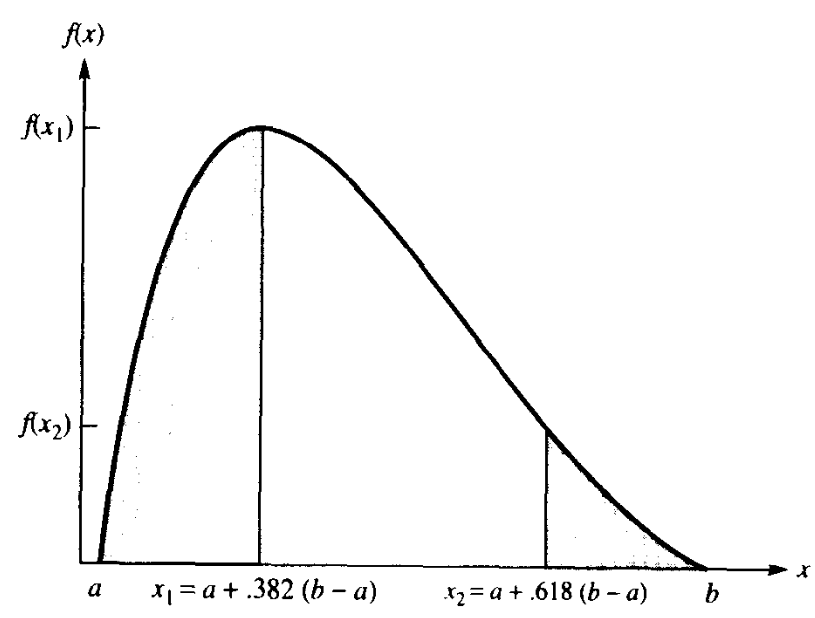
\includegraphics[height=.8\textheight{}]{gold.png}
  \end{figure}    
\end{frame}

\begin{frame}{Matlab中的搜索算法fminbnd}
  \begin{figure}
    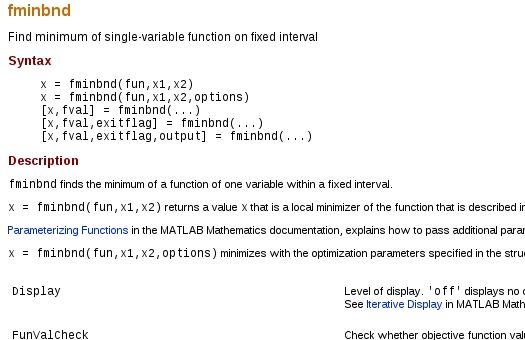
\includegraphics[height=.8\textheight{}]{fminbnd.png}
  \end{figure}      
\end{frame}

\begin{frame}{Matlab中的搜索算法fminsearch}
  \begin{figure}
    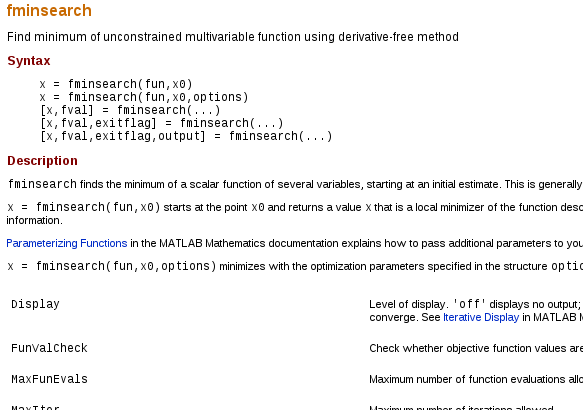
\includegraphics[height=.8\textheight{}]{fminsearch.png}
  \end{figure}      
\end{frame}

\end{document}

%%% Local Variables: 
%%% TeX-master: t
%%% TeX-engine: xetex
%%% End: 
